\section{Versuchsaufbau}
\label{sec:Versuchaufbau}
In diesem Kapitel werden alle in diesem Versuch verwendeten elektronischen Schaltungen für die Modulation als auch die Demodulation beschrieben und erläutert.
\subsection{Modulation}
\subsubsection{Primitive Modulatorschaltung mittels Diode}
\label{sec:Primitive_Modulatorschaltung_mittels_Diode}
Zur Realisierung einer Amplitudenmodulation wird eine Schaltung benötigt, die die Trägerspannung mit der Modulationsspannung multipliziert. Eine solcher Aufbau ist in Abbildung \ref{fig_10} dargestellt.

\begin{figure}
    \centering
    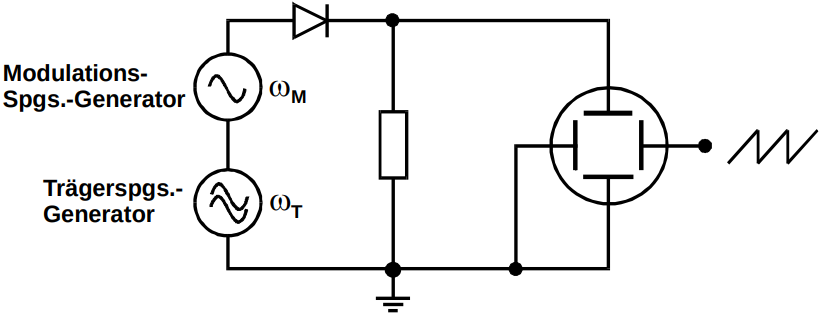
\includegraphics[width=0.55\textwidth]{ressources/A10.png}
    \caption{Aufbau einer Modulatorschaltung mittels Diode\cite{skript}.}
    \label{fig_10}
\end{figure}

Durch die nicht lineare Diodenkennlinie entstehen während der Multiplikation durch die Potenzreihenentwicklung neben dem benötigten Term $U_T \cdot U_M$ im zweiten Glied auch unerwünschte Therme höherer Ordnung der Träger- und Modulationsspannung. Dessen Frequenzen liegen außerhalb des Intervalls $[\omega_T-\omega_M, \omega_T+\omega_M]$ und können somit durch Bandfilter unterdrückt werden.

\subsubsection{Ringmodulator}
\label{sec:Ringmodulator}
Durch den sogenannten Ringmodulator, siehe Abbildung \ref{fig_02}, werden die bei der Schaltung im vorherigen Kapitel unerwünscht entstandenen Komponenten vermieden. Wie in Abbildung \ref{fig_02} dargestellt, sind die vier Dioden der Hauptbestandteil der Schaltung. 

\begin{figure}
    \centering
    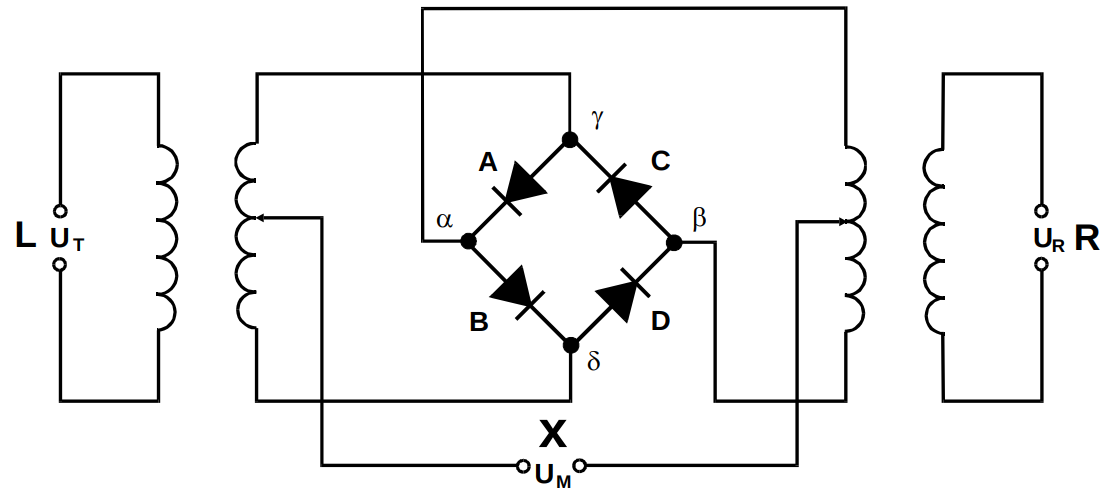
\includegraphics[width=0.55\textwidth]{ressources/A2.png}
    \caption{Aufbau eines Ringmodulatorschaltung \cite{skript}.}
    \label{fig_02}
\end{figure}

Durch diese wird eine Spannungsteiler an den Punkten $\alpha$ und $\beta$ realisiert, wodurch, bei baugleichen Dioden und ohne anliegender Modulationsspannung, keine Potentialdifferenz zwischen dem beiden besagten Punkten auftritt. Erst durch das Anlegen einer Modulationsspannung $U_M$ wird das Gleichgewicht gestört und die Teilungsverhältnisse der Dioden schwingen im Rhythmus von $U_M(t)$. Bei idealen Verhältnissen ist somit das Produkt der Eingangsspannungen proportional zur Ausgangsspannung. Aus diesem Grund entsteht bei dem Ringmodulator keine Trägerabstrahlung, weshalb nur die Seitenbänder entstehen.

\subsubsection{Frequenzmodulator mit geringem Frequenzhub}
\label{sec:Frequenzmodulator_mit_geringem_Frequenzhub}
Grundlage ist hierfür der in Kapitel \ref{sec:Ringmodulator} beschriebene Ringmodulator. Da durch diesen nur die Seitenbändern ohne Trägerabstrahlung erzeugt werden, muss die Trägerfrequenz mit einer Phasenverschiebung von $\pi/2$ gesondert hinzugefügt werden. Dieses wird, wie in Abbildung \ref{fig_03} dargestellt, über ein Laufzeitkabel von $\SI{250}{\ns}$ realisiert. 

\begin{figure}
    \centering
    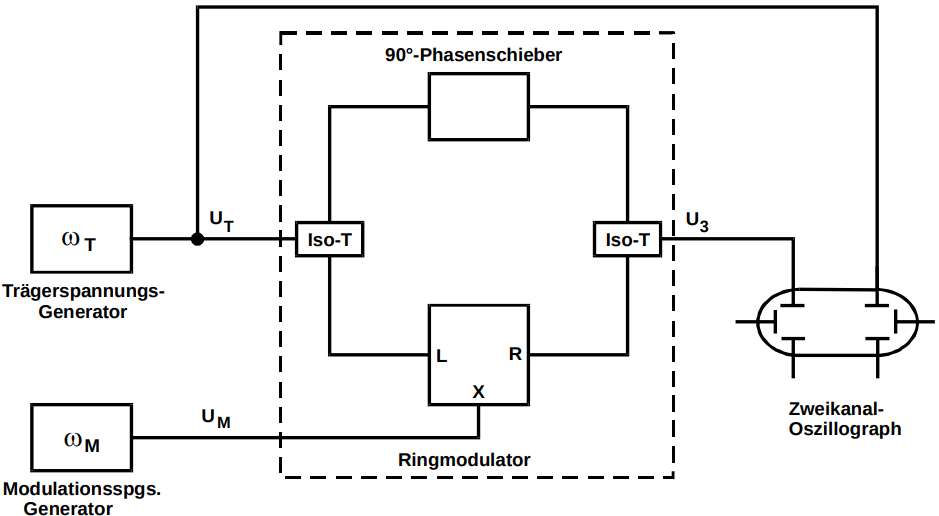
\includegraphics[width=0.55\textwidth]{ressources/A3.png}
    \caption{Darstellung einer Frequenzmodulatorschaltung mit Laufzeitkabel \cite{skript}.}
    \label{fig_03}
\end{figure}

Um die gewünschte Phasenverschiebung zu erhalten, kann über die zuvor passend eingestellte Periodendauer die benötigte Frequenz bestimmt werden.

\subsubsection{Phasenempfindlichkeit des Ringmodulators}
\label{sec:Phasenempfindlichkeit_der_Gleichrichterdiode}
Mit der folgenden Schaltung in Abbildung \ref{fig_11} wird durch die Variation der Frequenz und einem Laufzeitkabel die Phasenverschiebung erzeugt. 
\begin{figure}
    \centering
    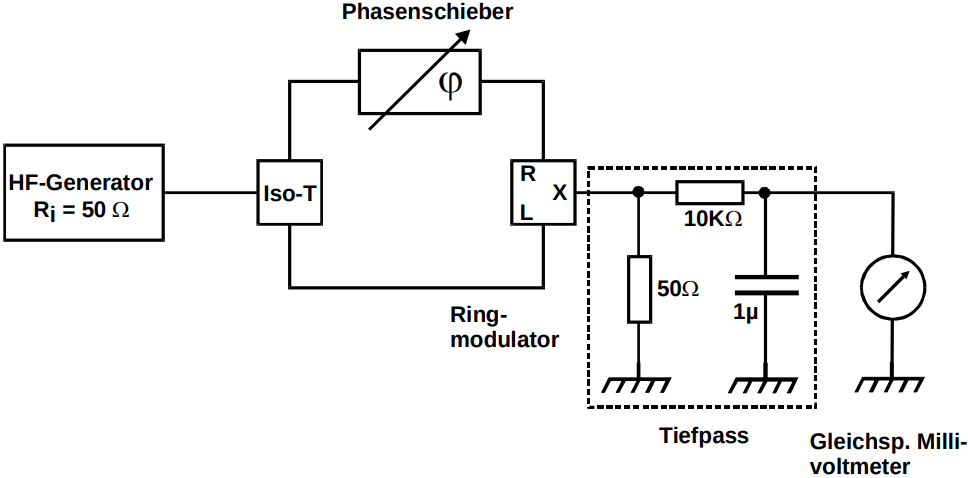
\includegraphics[width=0.55\textwidth]{ressources/A11.png}
    \caption{Darstellung einer Ringdiodenschaltung in Verbindung mit einem Laufzeitkabel und einem Amperemeter zu Überprüfung der Phasendifferenz \cite{skript}.}
    \label{fig_11}
\end{figure}
Über das Voltmeter wird die Spannung in Abhängigkeit der Frequenz dargestellt, wodurch die Proportionalität $U\approx\cos{(\phi)}$ überprüft wird. Hierfür wird die Abhängigkeit der Phase von der Frequenz verwendet.

\subsection{Demodulation}

\subsubsection{Demodulation amplitudenmodulierter Schwingungen}
\label{sec:Demodulation_amplitudenmodulieter_Schwingungen}
Zur Demodulation wird ebenfalls ein Ringmodulator verwendet. Wie in Abbildung \ref{fig_04} dargestellt, ist am Eingang L die modulierte Spannung und am Eingang R die Trägerspannung angelegt. 

\begin{figure}
    \centering
    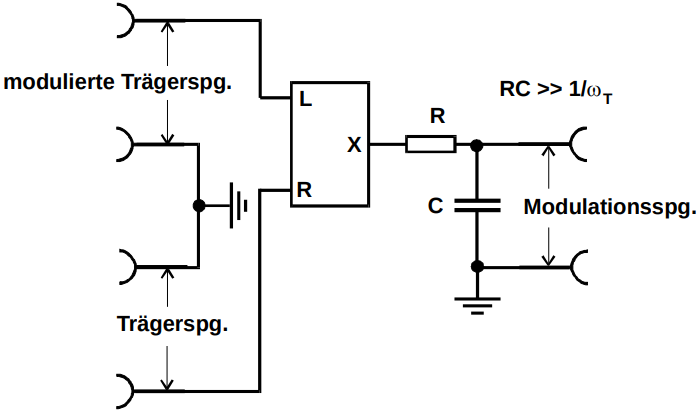
\includegraphics[width=0.55\textwidth]{ressources/A4.png}
    \caption{Darstellung eines Ringmodulators zur Demodulation einer amplitudenmodulierten Schwingung \cite{skript}.}
    \label{fig_04}
\end{figure}

Da die Frequenzen der Eingänge addiert und subtrahiert werden, ergeben sich aus den angelegten Frequenzen $\omega_T\pm\omega_M$ (Eingang L) und $\omega_T$ (Eingang R) am Ausgang X die Frequenzen $2\omega_T\pm\omega_M$ und $\omega_M$.

\subsubsection{Demodulator-Schaltung mit einer Gleichrichter-Diode}
\label{DSmeGD}
Ein weiteres Verfahren zur Demodulation einer Amplitudenmodulation besteht in der Verwendung einer Gleichrichterdiode mit geeignetem Tiefpass. Diese Schaltung findet Anwendung, wenn die ursprüngliche Trägerspannung nicht zur Demodulation zur Verfügung steht. Wie in Abbildung \ref{fig_05} dargestellt, werden durch die Diode sämtliche negativen Halbwellen der Signalspannung entfernt.

\begin{figure}
    \centering
    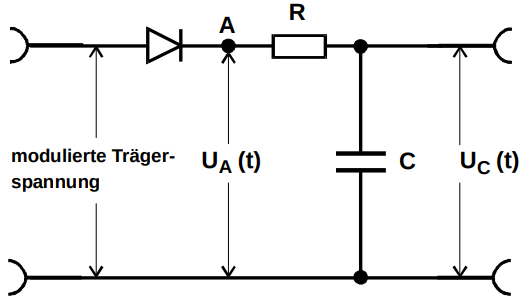
\includegraphics[width=0.55\textwidth]{ressources/A5.png}
    \caption{Darstellung einer Demodulationsschaltung mit Hilfe einer Gleichrichterdiode \cite{skript}.}
    \label{fig_05}
\end{figure}

Die in Abbildung \ref{fig_06} dargestellte Spannung am Punkt A enthält zu diesem Zeitpunkt hochfrequente Anteile der Form $\omega_T$, $2\omega_T$, $4\omega_T$ u.s.w. und $\omega_M$. Da die Beziehung $\omega_T>>\omega_M$ weiterhin gilt, kann die hohe Trägerfrequenz und deren Vielfache durch einen Tiefpass unterdrückt werden, sodass die in Abbildung \ref{fig_07} dargestellte Modulationsfrequenz extrahiert werden kann. 

\begin{figure}
    \centering
    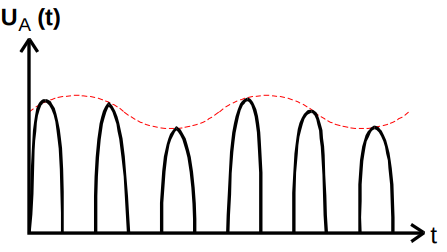
\includegraphics[width=0.45\textwidth]{ressources/A6.png}
    \caption{Darstellung der Spannung am Punkt A der Schaltung \ref{fig_05} \cite{skript}.}
    \label{fig_06}
\end{figure}

\begin{figure}
    \centering
    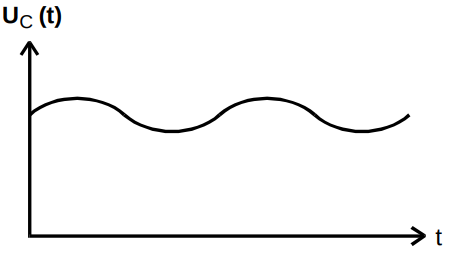
\includegraphics[width=0.45\textwidth]{ressources/A7.png}
    \caption{Darstellung der Spannung nach dem Tiefpass der Schaltung \ref{fig_05} \cite{skript}.}
    \label{fig_07}
\end{figure}

In der Realität ist die erhaltene Frequenz jedoch gegenüber der ursprünglichen Modulationsfrequenz verzerrt, da die Diode einen annähernd exponentiellen Kennlinienverlauf aufweist. Wird jedoch eine sehr kleine Modulationsfrequenz gewählt, kann die Kennlinie der Diode linear genähert werden und so eine Verzerrung vermindert werden.

\subsubsection{Demodulation frequenzmodulierter Schwingungen}
\label{sec:Demodulation_frequenzmodulieter_Schwingungen}
Im ersten Teil der Demodulation findet die Umwandlung in eine amplitudenmodulierte Schwingung statt. Dieses wird durch einen LC-Schwingkreis realisiert, wie in Abbildung \ref{fig_12} zu sehen. 

\begin{figure}
    \centering
    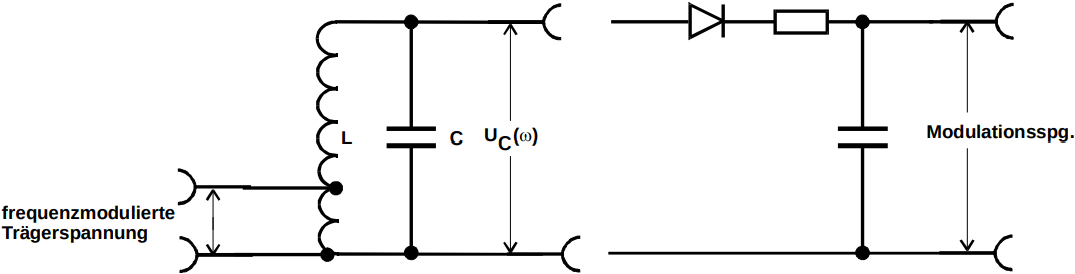
\includegraphics[width=0.80\textwidth]{ressources/A12.png}
    \caption{Darstellung eines LC-Schwingkreises mit dem die frequenzmodulierte Schwingung in eine amplitudenmodulierte Schwingung überführt wird. \cite{skript}.}
    \label{fig_12}
\end{figure}


Aus diesem Grund ist die Resonanzfrequenz der Schaltung so gewählt, dass die Trägerfrequenz auf der Flanke der Resonanzkurve liegt (siehe Abbildung \ref{fig_08}). Ändert sich Momentanfrequenz der Schwingung, so entsteht am Ausgang der Schaltung eine hochfrequente Spannung, die keine konstante Amplitude mehr aufweist, sondern deren Amplitude im Rhythmus der Modulationsfrequenz schwingt. Im zweiten Schritt ist die Demodulation der amplitudenmodulierten Schwingung durch die in Kapitel \ref{sec:Demodulation_amplitudenmodulieter_Schwingungen} oder \ref{DSmeGD} vorgestellte Methoden durchzuführen. 

\begin{figure}
    \centering
    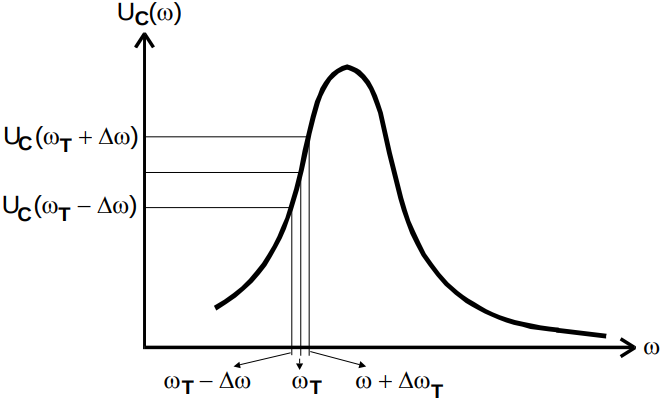
\includegraphics[width=0.55\textwidth]{ressources/A8.png}
    \caption{Darstellung der Resonanzkurve des LC-Schwingkreises und dem Frequenzspektrum der modulierten Schwingung auf dessen Flanke \cite{skript}.}
    \label{fig_08}
\end{figure}
